% !TEX root = ./main.tex
\documentclass[a4paper]{article}
% Course language: use [english] or [german].
\usepackage[german]{ajnotes}
\title{\textbf{Mikrooekonomik — Praeferenzen}}
\begin{document}
    \maketitle
    % Attach the given problem sheet: drop it in this folder as sheet.pdf and
    % un-comment the next line (pdfpages is already loaded by the preamble).
    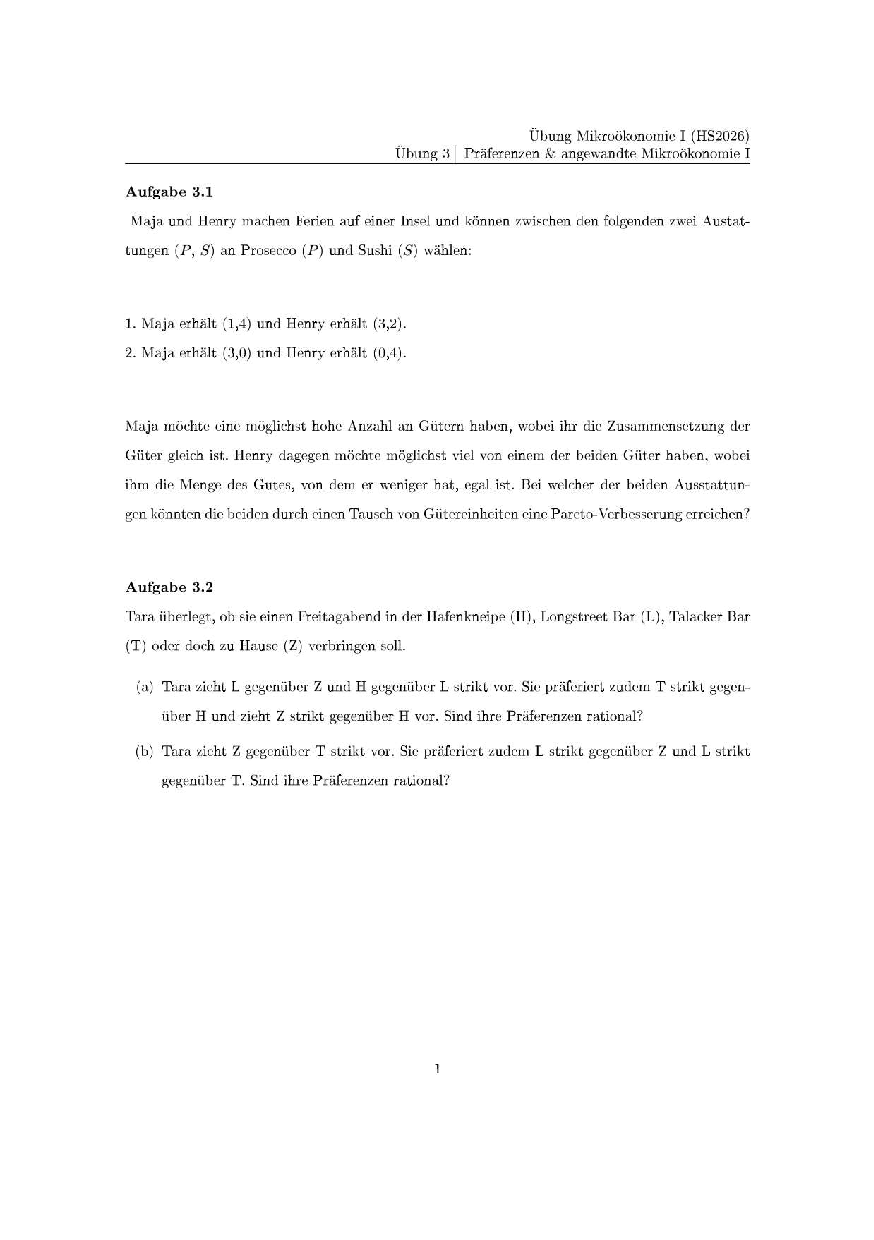
\includepdf[pages=-]{sheet.pdf}
    \exercise{3.1}
    \textbf{Als funktionen}
    \begin{equation}
        U_m(P,S) = P + S 
    \end{equation}
    \begin{equation}
        U_H (P,S) = max\left\{P,S\right\}
    \end{equation}
    1. Weil nur hier ist ein Gütertausch möglich die den Beiden besser stellt. Bei einem Tausch von 1 P gegen 2 S sind beide Bedingungen erfüllt und wenigsten 1 Nutzen, den Henrys, erhöht.
    \exercise{3.2}
    \subexercise{a}
    Tara:
    \begin{equation}
      T \succ H \succ L \succ Z 
    \end{equation}
    Nein, weil Z gegenüber H präferieren einen Widerspruch zu $H \succ L \succ Z $. Transitivität wird verletzt.
    \subexercise{b}
    \begin{equation}
       L \succ Z \succ T 
    \end{equation}
    Ja ist rational. Keinen Widerspruch, Transitivität und 
    \textbf{NEIN, weil Vollständigkeit verletzt. H wird nicht Berücksichtigt}
    
    \exercise{3.3}
    max 2 
    \subexercise{a}
    \textbf{NEIN}, die Ausgewogenheit wird Präferiert (Konvexität) aber Bündel (0,1) ist indifferent zu (0,0) obwohl die Menge grösser ist. (Nichtsättigung verletzt)
    \subexercise{b}
    Nein, (0,2) wird über (1,1) präferiert (Konvexität verletzt). Nichtsättigung bleibt erhalten.
    \exercise{3.4}
    \subexercise{a}
    Markt ohne Geldvermittlung \footnote{Dies als Markt zu bezeichnen zeigt die Distanz zur spezifischen Realität und die Betrachtung des Geldes als ein neutrales Werkzeug, das sich nur den Willen der Menschen anspasst und keine eigene spezifische interne Logik und objektive Funktionsweise hat.}
    \subexercise{b}
    \begin{itemize}
        \item Wie sind präferenzen bei der Partnerwahl von Frauen und Männer.
        \item 
    \end{itemize}
    \subexercise{c}
    \begin{itemize}
        \item Universität Stundenten wurden Zufällig ausgewahlt für einen Speed-Dating experiment. Je 4 min runden
        \item 
    \end{itemize}

\end{document}
